\let\negmedspace\undefined
\let\negthickspace\undefined
\documentclass[journal]{IEEEtran}
\usepackage[a5paper, margin=10mm, onecolumn]{geometry}
%\usepackage{lmodern} % Ensure lmodern is loaded for pdflatex
\usepackage{tfrupee} % Include tfrupee package

\setlength{\headheight}{1cm} % Set the height of the header box
\setlength{\headsep}{0mm}     % Set the distance between the header box and the top of the text

\usepackage{gvv-book}
\usepackage{gvv}
\usepackage{cite}
\usepackage{amsmath,amssymb,amsfonts,amsthm}
\usepackage{algorithmic}
\usepackage{graphicx}
\usepackage{textcomp}
\usepackage{xcolor}
\usepackage{txfonts}
\usepackage{listings}
\usepackage{enumitem}
\usepackage{mathtools}
\usepackage{gensymb}
\usepackage{comment}
\usepackage[breaklinks=true]{hyperref}
\usepackage{tkz-euclide} 
\usepackage{listings}
% \usepackage{gvv}                                        
\def\inputGnumericTable{}                                 
\usepackage[latin1]{inputenc}                                
\usepackage{color}                                            
\usepackage{array}                                            
\usepackage{longtable}                                       
\usepackage{calc}                                             
\usepackage{multirow}                                         
\usepackage{hhline}                                           
\usepackage{ifthen}                                           
\usepackage{lscape}
\usepackage{circuitikz}



\author{EE25BTECH11041-Naman Kumar }
\graphicspath{./figs/}

\begin{document}
\begin{center}
    \huge{4.3.30}\\
    \large{EE25BTECH11041 - Naman Kumar}
\end{center}
Question:\\
Find the equation of the line which passes through the point $(-4, 3)$ and the portion of the line intercepted between the axes is divided internally in ratio 5:3 by this point.\\
\solution \\
Let the intercept points be
\begin{align}
    \vec{P}=a\vec{e_1},\vec{Q}=b\vec{e_2} \\\vec{e_1}=\begin{pmatrix}1\\0\end{pmatrix}, \vec{e_2}=\begin{pmatrix}0\\1\end{pmatrix}, \text{a and b are constants}
\end{align}
and
\begin{align}
    \vec{R}=\begin{pmatrix}-4\\3\end{pmatrix}=-4e_1+3e_2
\end{align}
be the given point.\\
Using
\begin{align}
    \vec{R}=\frac{k\vec{Q}+\vec{P}}{k+1} \label{section}\\
    \vec{R}=\frac{5\times b\vec{e_2}+3\times a\vec{e_1}}{8}\\
    -4\vec{e_1}+3\vec{e_2}=\frac{5\times b\vec{e_2}+3\times a\vec{e_1}}{8}\\
    -32\vec{e_1}+24\vec{e_2}=3a\vec{e_1}+5b\vec{e_2} \label{points}
\end{align}
General equation of line
\begin{align}
    \vec{x}=\vec{h}+c\vec{m}
\end{align}
Where\\
\begin{table}[h!]
    \centering
    \begin{tabular}{|c|c|}
        \hline
        Point & Coordinates \\
        \hline
	    $A$ & $\myvec{1\\-1}$ \\
	    $B$ & $\myvec{-4\\2k}$ \\
	    $C$ & $\myvec{-k\\-5}$ \\
        \hline
    \end{tabular}
    \caption{Vertices of $\triangle ABC$ before substituting $k$}
    \label{tab:triangle_k}
\end{table}

\newpage
Slope is
\begin{align}
\vec{m}=\vec{Q}-\vec{P}\\
\end{align}
let $\vec{h}=\vec{P}$\\
So, Equation of line is
\begin{align}
    \vec{x}=\vec{h}+c\vec{m}\\
    \vec{x}=\vec{P}+c(\vec{Q}-\vec{P})
\end{align}
Putting values of $\vec{Q},\vec{P}$
\begin{align}
    \vec{x}=a\vec{e_1}+c(b\vec{e_2}-a\vec{e_1})
\end{align}
Comparing terms in \eqref{points} for values of a and b
\begin{align}
    \vec{x}=\frac{-32}{3}\vec{e_1}+c(\frac{24}{5}\vec{e_2}-\frac{-32}{3}\vec{e_1})
\end{align}
Therefore Final equation is
\begin{align}
\begin{pmatrix}x\\y\end{pmatrix}=\begin{pmatrix}\frac{-32}{3}\\0\end{pmatrix}+k\begin{pmatrix}\frac{32}{3}\\ \frac{24}{5}\end{pmatrix}
\end{align}
\begin{figure}[H]
    \centering
    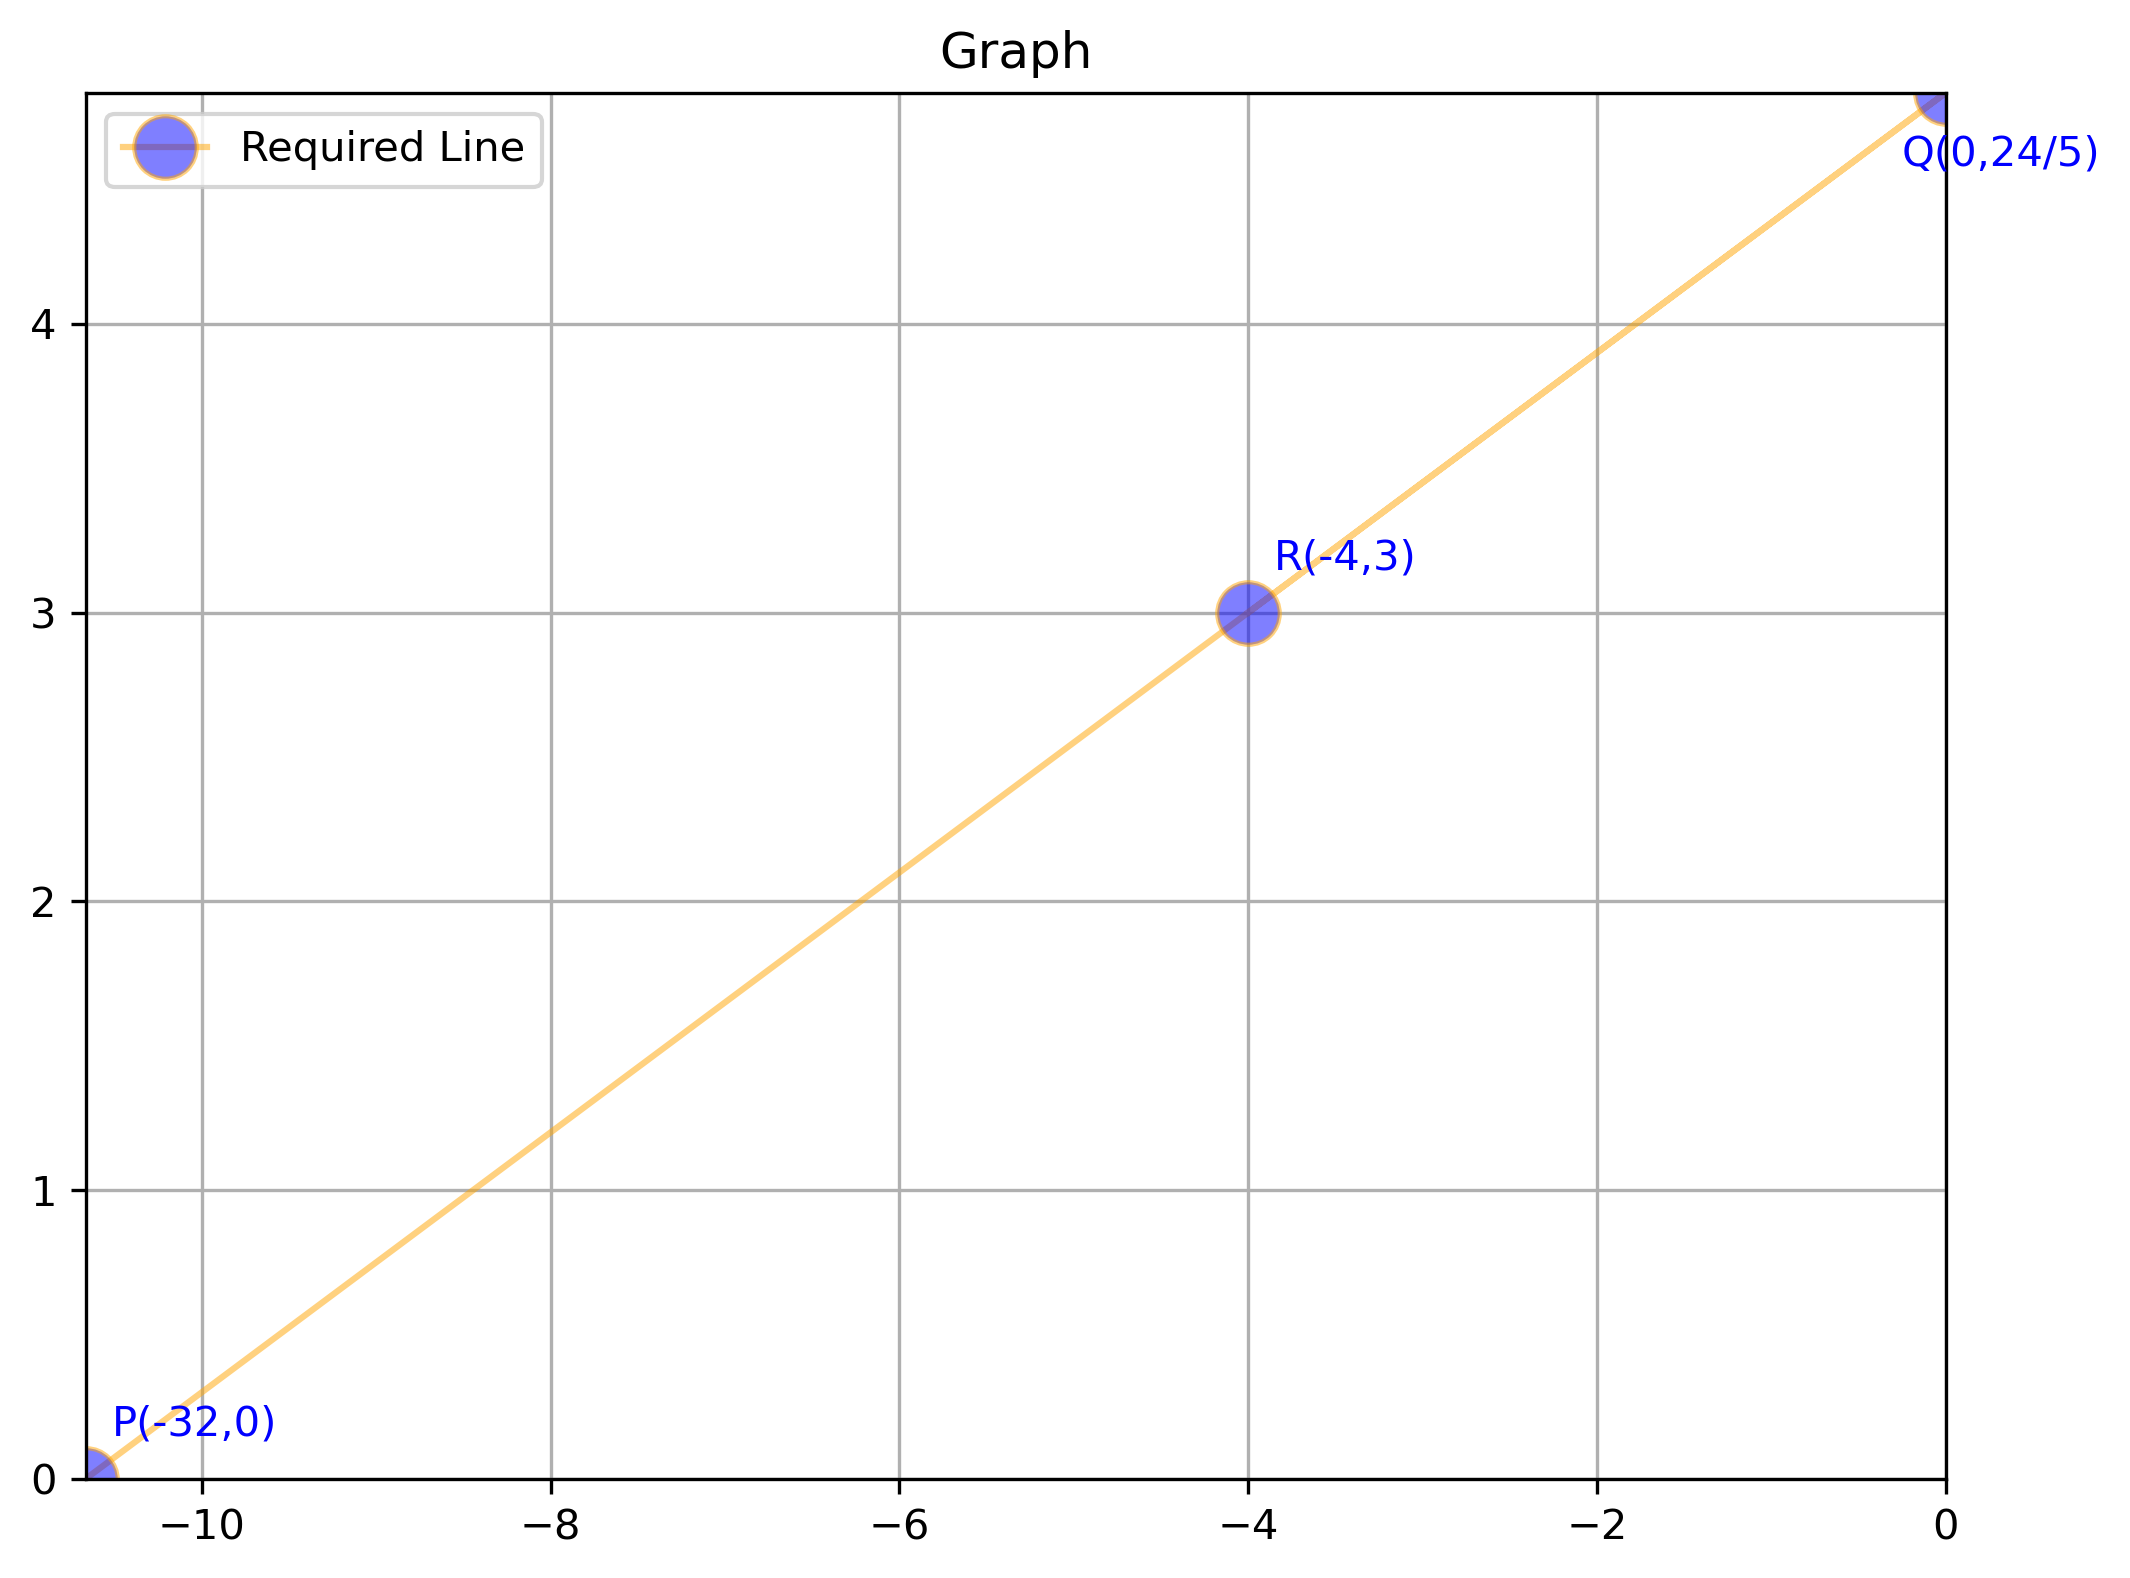
\includegraphics[width=\columnwidth]{figs/figure.png}
    \label{fig:placeholder}
\end{figure}
\end{document}
